%\documentclass[notes]{beamer}       % print frame + notes
% \documentclass[notes=only]{beamer}   % only notes
\documentclass{beamer}  

\usepackage{wrapfig}
\usepackage{amsmath,amssymb}
%\usepackage[dvipsname]{xcolor}
\usepackage{tikz}
\usepackage{tikz-cd}
\usepackage{graphicx}

\usetikzlibrary{shapes.geometric}

\tikzset{pics/.cd,
opencube/.style args={#1/#2/#3}{code={
\coordinate (O) at (0,0,0);
\coordinate (A) at (0,#2,0);
\coordinate (B) at (0,#2,#3);
\coordinate (C) at (0,0,#3);
\coordinate (D) at (#1,0,0);
\coordinate (E) at (#1,#2,0);
\coordinate (F) at (#1,#2,#3);
\coordinate (G) at (#1,0,#3);
%% Background
\draw[black,dotted] (O) -- (A);
\draw[black,dotted] (O) -- (C);
\draw[black,dotted] (O) -- (D);
% Forground
\draw[black,dashed] (A) -- (E) -- (F) -- (B) -- cycle;
\draw[black,dashed] (E) -- (D) -- (G) -- (C) -- (B);
\draw[black,dashed] (F) -- (G);

%\draw[black,dashed, blue] (O) -- (A) -- (E) -- (D) -- cycle;
%\draw[black,dashed] (O) -- (A) -- (B) -- (C) -- cycle;
%\draw[black,dashed] (D) -- (E) -- (F) -- (G) -- cycle;
%\draw[black,dashed] (C) -- (B) -- (F) -- (G) -- cycle;
%\draw[black,dashed] (A) -- (B) -- (F) -- (E) -- cycle;

}}}

\tikzset{pics/.cd,
linecube/.style args={#1/#2/#3/#4}{code={
\coordinate (OO) at (0,0,0);
\coordinate (AA) at (0,#2,0);
\coordinate (BB) at (0,#2,#3);
\coordinate (CC) at (0,0,#3);
\coordinate (DD) at (#1,0,0);
\coordinate (EE) at (#1,#2,0);
\coordinate (FF) at (#1,#2,#3);

\coordinate (GG) at (#1,0,#3);
%% Background
\draw[black,dashed] (OO) -- (AA);
\draw[black,dashed] (OO) -- (CC);
\draw[black,dashed] (OO) -- (DD);

\node at (0.5*#1,0.5*#2,0.5*#3) {#4};

% Foreground
\draw[black] (AA) -- (EE) -- (FF) -- (BB) -- cycle;
\draw[black] (EE) -- (DD) -- (GG) -- (CC) -- (BB);
\draw[black] (FF) -- (GG);

%\draw[black,dashed, blue] (O) -- (A) -- (E) -- (D) -- cycle;
%\draw[black,dashed] (O) -- (A) -- (B) -- (C) -- cycle;
%\draw[black,dashed] (D) -- (E) -- (F) -- (G) -- cycle;
%\draw[black,dashed] (C) -- (B) -- (F) -- (G) -- cycle;
%\draw[black,dashed] (A) -- (B) -- (F) -- (E) -- cycle;

}}}


\tikzset{pics/.cd,
shadedcube/.style args={#1/#2/#3/#4/#5}{code={
\coordinate (O) at (0,0,0);
\coordinate (A) at (0,#2,0);
\coordinate (B) at (0,#2,#3);
\coordinate (C) at (0,0,#3);
\coordinate (D) at (#1,0,0);
\coordinate (E) at (#1,#2,0);
\coordinate (F) at (#1,#2,#3);
\coordinate (G) at (#1,0,#3);
\draw[black,fill=#4!80] (O) -- (C) -- (G) -- (D) -- cycle;
\draw[black,fill=#4!30] (O) -- (A) -- (E) -- (D) -- cycle;
\draw[black,fill=#4!10] (O) -- (A) -- (B) -- (C) -- cycle;
\draw[black,fill=#4!20,opacity=0.8] (D) -- (E) -- (F) -- (G) -- cycle;
\draw[black,fill=#4!20,opacity=0.6] (C) -- (B) -- (F) -- (G) -- cycle;
\draw[black,fill=#4!20,opacity=0.8] (A) -- (B) -- (F) -- (E) -- cycle;
\node at (0.5*#1,0.5*#2,0.5*#3) {#5};
}}}
\tikzset{pics/.cd,
gridcube/.style args={#1/#2/#3/#4/#5/#6/#7}{code={
\coordinate (O) at (0,0,0);
\coordinate (A) at (0,#2,0);
\coordinate (B) at (0,#2,#3);
\coordinate (C) at (0,0,#3);
\coordinate (D) at (#1,0,0);
\coordinate (E) at (#1,#2,0);
\coordinate (F) at (#1,#2,#3);
\coordinate (G) at (#1,0,#3);

% Foreground
\draw[fill=#7!20] (A) -- (E) -- (F) -- (B) -- cycle;
\draw[fill=#7!40] (E) -- (F) -- (G) -- (D) -- cycle;
\draw[fill=#7!30] (B) -- (F) -- (G) -- (C) -- cycle;
%\draw[black] (E) -- (D) -- (G) -- (C) -- (B);
%\draw[black] (F) -- (G);

% lines
\foreach \ll in {1,...,#4} {
    \draw[black] (#1/#4*\ll,#2,0) -- (#1/#4*\ll,#2,#3) -- (#1/#4*\ll,0,#3);
}
\foreach \ll in {1,...,#5} {
    \draw[black] (0,#2/#5*\ll,#3) -- (#1, #2/#5*\ll,#3) -- (#1,#2/#5*\ll,0);
}
\foreach \ll in {1,...,#6} {
    \draw[black] (0,#2,#3/#6*\ll) -- (#1,#2,#3/#6*\ll) -- (#1,0,#3/#6*\ll);
}

}}}

%\pgfmathsetmacro{\xx}{0.5}

\mode<presentation>
% \setbeameroption{hide notes}
{
  %\usetheme{Madrid}
  \usetheme{metropolis}
% CSU COLORS
  \definecolor{csugreen}{HTML}{1C674F}
  \definecolor{csugold}{HTML}{B78E00}
    \definecolor{csured}{HTML}{E02F11}

  \definecolor{greenmain}{HTML}{00AF64}
  \definecolor{brick}{rgb}{.85,.1,.2}
  \colorlet{greenstruct}{greenmain!87.5!black}
  \usecolortheme[named=csugreen]{structure}
  % Change this in order to make the presentation look
  % different. Works just like a powerpoint template. 
  % Have your RA mess around until it looks nice.
  \setbeamercovered{dynamic}

  \useinnertheme{rectangles}
  
 %Other colors.

%   \definecolor{bluemain}{HTML}{0B61A4}
%   \definecolor{orangemain}{HTML}{AA6600}
%   \definecolor{redmain}{HTML}{E02F11}
%   \definecolor{redlight}{HTML}{FF9B73}
%   \definecolor{orangelight}{HTML}{FFC373}
%   \definecolor{cmugray}{RGB}{104,104,104}
%   \definecolor{cmulightgray}{RGB}{238,238,238}
%   \setbeamercolor{block body}{bg=cmulightgray}
%   \setbeamercolor{talktitle}{bg=csugreen,fg=white}
%   \setbeamercolor{block title alerted}{bg=csugold}
%   \setbeamercolor{block body alerted}{bg=orangelight}

}
\renewcommand{\footnoterule}{}
\renewcommand{\hat}[1]{\widehat{#1}}
\newcommand{\sourcenum}[3]{$^{\textcolor{bluemain} #1}$\let\thefootnote\relax
  \footnotetext{\begin{flush#2}\textcolor{bluemain}
      {\tiny $^{#1}$ #3}\end{flush#2}}} 
\newcommand{\source}[2]{\let\thefootnote\relax\footnotetext{\begin{flush#1}
      \textcolor{bluemain}{\tiny Source: #2}\end{flush#1}}}  


\DeclareMathOperator{\Span}{Span}
\DeclareMathOperator{\Pres}{Pres}
\DeclareMathOperator{\End}{End}
\newcommand{\bmto}{\rightarrowtail}

\usepackage{wasysym} 
\newcommand{\den}[1]{\Leftcircle\hspace*{-1mm}#1\hspace*{-1mm} \Rightcircle}
\usepackage{listings}

\begin{document}

\title{Group isomorphism is nearly-linear time for most
orders\\ {\small IEEE Foundations On Computer Science FOCS 2021}}
\author{Heiko Dietrich\\ Monash University, Australia\\[10pt] James B. Wilson (presenting)\\ Colorado State University, USA}
\date{February 8, 2022}

\maketitle

%%%%%%%%%%%%%%%%%%%%%%%%%%%%%%%%%%%%%%%%%%%%%%%%%%%%%%%%
\section{Motivation}

\begin{frame}[containsverbatim]{Outward Facing Motive: honest data types}
Where in this... 
%\includegraphics[height=0.3\textheight]{Algo.jpg}    
...or this...
%\includegraphics[height=0.3\textheight]{java-api.png}\\
...do we send people to get get help with this... 

\bigskip
\begin{lstlisting}[mathescape=true,language=Java,basicstyle=\ttfamily,commentstyle=\color{csugreen},keywordstyle=\color{blue}]
boolean equals(Object that) {
    // <this> can transform into <that>?
    ???
}
\end{lstlisting}
    
\vfill
A type without proper equality is just a container (list/tree/array/struct...)
\end{frame}

\begin{frame}[containsverbatim]{Inward facing Motive: equalivance surveys complexity}


\end{frame}

\begin{frame}{Schreier-Sims}

    \begin{block}{Problem: Transport}
    \begin{description}
        \item[Given:] A set $\Omega$, allowed permutations $X$, $\omega,\omega'\in\Omega$
        \item[Return:] decide if a string $g$ over $X$ maps $\omega$ to $\omega'$, 
        written $\omega^{g}=\omega'$, and give all such $g$.\footnote{Give words $W$ over $X$
        so that $\omega^h=\omega'$ implies $h=wg$ for a string $w$ over $W$.}
    \end{description}
    \end{block}
\end{frame}



\begin{frame}[fragile]{String Isomorphism}

\only<1>{
``eighth'' == ``$\epsilon\iota\gamma\tau\eta\tau\eta$''. 
\begin{block}{String Isomorphism (Internet Edition)}
\begin{minipage}{0.6\textwidth}
\begin{description}
    \item[Given] $s:I\to \Sigma$, $t:I\to \Delta$
    \item[Return] bijection $\pi:\Sigma\to \Delta$, $\pi(s_{i})=t_i$.
\end{description}
\end{minipage}
\hfill 
\begin{minipage}{0.3\textwidth}
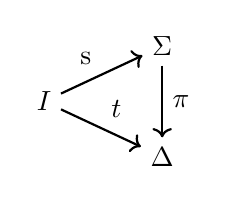
\begin{tikzpicture}
\node (I) at (-1,0) {$I$};
\node (S) at (0.5,0.7) {$\Sigma$};
\node (T) at (0.5,-0.7) {$\Delta$};
\draw[thick,->] (I) to[midway, "s"] (S);
\draw[thick,->] (I) to[midway, "$t$"] (T);
\draw[thick,->] (S) to[midway, "$\pi$"] (T);
\end{tikzpicture}
\end{minipage}
\end{block}
\textbf{Complexity:} $O(n)$, homework assignment.
}
\only<2>{
    ``eighth'' == ``height''
\begin{block}{String Isomorphism (Complexity Edition)}
    \begin{minipage}{0.6\textwidth}
        \begin{description}
    \item[Given] strings $s:I\to \Sigma$, $\tilde{s}:\tilde{I}\to \Sigma$
    \item[Return] bijection $\pi:I\to \tilde{I}$, $s_{\pi(i)}=t_i$.
\end{description}
\end{minipage}
\hfill 
\begin{minipage}{0.3\textwidth}
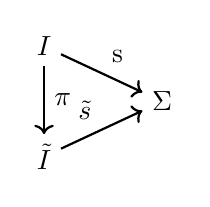
\begin{tikzpicture}
\node (I) at (-0.5,0.7) {$I$};
\node (J) at (-0.5,-0.7) {$\tilde{I}$};
\node (S) at (1,0) {$\Sigma$};
\draw[thick,->] (I) to[midway, "s"] (S);
\draw[thick,->] (J) to[midway, "$\tilde{s}$"] (S);
\draw[thick,->] (I) to[midway, "$\pi$"] (J);
\end{tikzpicture}
\end{minipage}
\end{block}
\textbf{Complexity:} Babai Quasipolynomial $n^{O((\log n)^c)}$.\\
Decades of work by Babai, Luks, Weisfeiler-Leman and others.
\vfill
(\textsc{GraphIso}$\leq_P$ \textsc{StringIso})
}
\end{frame}

%========================================================
\section{Isomorphism of Tables}

\begin{frame}[fragile]{Code Equivalence}

\begin{block}{Code Equivalence}
\begin{minipage}{0.6\textwidth}
\begin{description}
    \item[Given] $s:I\time J\to \Sigma$, $\tilde{s}:\tilde{S}\times \tilde{J}\to \Sigma$
    \item[Return]  $\exists$ bijections $\sigma:I\to \tilde{I}$ and $\tau:J\to \tilde{J}$
    $s_{\pi(i)\tau(j)} & = \tilde{s}_{ij}$
\end{description}
\end{minipage}
\hfill 
\begin{minipage}{0.3\textwidth}
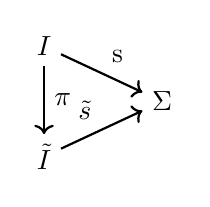
\begin{tikzpicture}
\node (I) at (-0.5,0.7) {$I$};
\node (J) at (-0.5,-0.7) {$\tilde{I}$};
\node (S) at (1,0) {$\Sigma$};
\draw[thick,->] (I) to[midway, "s"] (S);
\draw[thick,->] (J) to[midway, "$\tilde{s}$"] (S);
\draw[thick,->] (I) to[midway, "$\pi$"] (J);
\end{tikzpicture}
\end{minipage}

\end{block}

\end{frame}

%==============================================================================
\section{Is it a Group Table?}

\begin{frame}{IsGroup in Nearly Linear Time}
\begin{block}{Theorem Rajagopalan-Schulman, 2000}
    Given $*:[n]\times [n]\to [n]$, test associativity in nearly-linear time 
    $\tilde{O}(n^2)$ in RAM model 
    (constant time ops and memory access).
    Also can test if a group.
\end{block}
\begin{block}{Corollary}
Nearly Quadratic-time $\tilde{O}(n^4)$ on multi-tape Turing Machine (TM).
\end{block}

\pause
\begin{block}{Theorem Dietrich-W.}
    Given $*:[n]\times [n]\to [n]$,
    test if a group in time nearly-linear time
    $\tilde{O}(n^2)$ on deterministic multi-tape TM.
    % \footnote{One tape of input length $\ell\in O(n^2)$,
    % and another of length $O(\sqrt{\ell})$.}
\end{block}

\end{frame}

\begin{frame}{IsGroup Sketch}
\tikzset{
mybox/.style={
    inner sep=0pt,
    text width=5mm,
    text height=5mm,
    align=center,
    }
}
\begin{tikzpicture}
\node[fill=blue!0, label=center:1,mybox] at  ( 0mm, -0mm) {};
\node[fill=blue!20,label=center:2,mybox] at  ( 5mm, -0mm) {};
\node[fill=blue!20,label=center:3,mybox] at  (10mm, -0mm) {};
\node[fill=blue!30,label=center:4,mybox] at  (15mm, -0mm) {};
\node[fill=blue!40,label=center:5,mybox] at  (20mm, -0mm) {};
%
\node[fill=blue!10,label=center:2,mybox] at  ( 0mm, -5mm) {};
\node[fill=blue!30,label=center:4,mybox] at  ( 5mm, -5mm) {};
\node[fill=blue!0, label=center:1,mybox] at  (10mm, -5mm) {};
\node[fill=blue!40,label=center:5,mybox] at  (15mm, -5mm) {};
\node[fill=blue!20,label=center:3,mybox] at  (20mm, -5mm) {};
%
\node[fill=blue!20,label=center:3,mybox] at  ( 0mm,-10mm) {};
\node[fill=blue!40,label=center:5,mybox] at  ( 5mm,-10mm) {};
\node[fill=blue!30,label=center:4,mybox] at  (10mm,-10mm) {};
\node[fill=blue!10,label=center:2,mybox] at  (15mm,-10mm) {};
\node[fill=blue!0, label=center:1,mybox] at  (20mm,-10mm) {};
%
\node[fill=blue!30,label=center:4,mybox] at  ( 0mm,-15mm) {};
\node[fill=blue!0, label=center:1,mybox] at  ( 5mm,-15mm) {};
\node[fill=blue!40,label=center:5,mybox] at  (10mm,-15mm) {};
\node[fill=blue!20,label=center:3,mybox] at  (15mm,-15mm) {};
\node[fill=blue!10,label=center:2,mybox] at  (20mm,-15mm) {};
%
\node[fill=blue!40,label=center:5,mybox] at  ( 0mm,-20mm) {};
\node[fill=blue!20,label=center:3,mybox] at  ( 5mm,-20mm) {};
\node[fill=blue!10,label=center:2,mybox] at  (10mm,-20mm) {};
\node[fill=blue!0, label=center:1,mybox] at  (15mm,-20mm) {};
\node[fill=blue!30,label=center:4,mybox] at  (20mm,-20mm) {};
\end{tikzpicture}

\end{frame}


\begin{frame}{IsGroup}

\begin{tikzpicture}
    \node at (0,0) {$
        \begin{array}{|c|ccccc|}
        \hline
        \bullet & 1 & 2 & 3 & 4 & 5\\
        \hline
        1 & 1 & 2 & 3 & 4 & 5\\
        2 & 2 & 1 & 4 & 5 & 3\\
        3 & 3 & 5 & 1 & 2 & 4\\
        4 & 4 & 3 & 5 & 1 & 2\\
        5 & 5 & 4 & 2 & 3 & 1\\
        \hline
        \end{array}   
    $};
    \visible<2->{
    \node at (6,0) {$
        \rho(2)  = 
        \begin{array}{|ccccc|}
        \hline
            1 & 2 & 3 & 4 & 5 \\
        \hline 
            2 & 1 & 4 & 5 & 3 \\
        \hline \end{array}    
        =
        (1,2)(3,5,4)
    $};
    };
    \visible<3->{
    \node at (0,-3) {\begin{tikzpicture}
        \node[circle,draw] (1) at (0,0) {1};
        \node[circle,draw] (2) at (2,0) {2};
        \draw[->,thick] (1) to[bend left=30] (2);
        \draw[->,thick] (2) to[bend left=30] (1);
    \end{tikzpicture}};
    \node at (0,-4.5) {$G_{1}=\langle (354)\rangle$};
    };
    \visible<4->{
    \node at (3,-3) {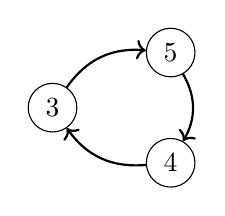
\begin{tikzpicture}
        \node[circle,draw] (3) at (-1,0) {3};
        \node[circle,draw] (4) at (0.5,0.7) {5};
        \node[circle,draw] (5) at (0.5,-0.7) {4};

        \draw[->,thick] (3) to[bend left=30] (4);
        \draw[->,thick] (4) to[bend left=30] (5);
        \draw[->,thick] (5) to[bend left=30] (3);
    \end{tikzpicture}};
    \node at (3,-4.5) {$G_{13}=\{1\}$};
    };
    \visible<5>{
    \node[text width=4cm] at (8,-3) {$|G|=[G:G_1][G_1:G_{13}]$\\ $~=2\cdot 3=6$.\\  Should be 5,\\ not a group.};
    };
\end{tikzpicture}

\end{frame}

    
\begin{frame}{IsGroup}
    \begin{tikzpicture}
        \node at (0,0) {$
        \begin{array}{|c|ccccc|}
        \hline
        * & 1 & 2 & 3 & 4 & 5 \\
        \hline 
        1 & 1 & 2 & 3 & 4 & 5 \\ 
        2 & 2 & 4 & 1 & 5 & 3 \\
        3 & 3 & 5 & 4 & 2 & 1 \\
        4 & 4 & 1 & 5 & 3 & 2 \\
        5 & 5 & 3 & 2 & 1 & 4 \\
        \hline \end{array}    
        $};
        \visible<2->{
        \node at (6,0) {$
            \rho(2)  = 
            \begin{array}{|ccccc|}
            \hline
                1 & 2 & 3 & 4 & 5 \\
            \hline 
                2 & 4 & 1 & 5 & 3 \\
            \hline \end{array}    
            =
            (1,2,4,5,3)
        $};
        };
        \visible<3->{
        \node at (0,-3) {\begin{tikzpicture}
            \node[circle,draw] (1) at (1,0) {1};
            \node[circle,draw] (2) at (0.3,0.8) {2};
            \node[circle,draw] (3) at (-0.6,0.5) {3};
            \node[circle,draw] (4) at (-0.6,-0.5) {4};
            \node[circle,draw] (5) at (0.3,-0.8) {5};

            \draw[->,thick] (1) to[bend right=30] (2);
            \draw[->,thick] (2) to[bend left=30] (4);
            \draw[->,thick] (4) to[bend right=30] (5);
            \draw[->,thick] (5) to[bend right=30] (3);
            \draw[->,thick] (3) to[bend right=30] (1);
        \end{tikzpicture}};
        \node at (0,-4.5) {$|G|=[G:G_{1}|=5$};
        };
        \visible<4>{
        \node[text width=4cm] at (7,-3) {$
        \begin{array}{|c|ccccc|}
        \hline
        * & 1 & 2 & 3 & 4 & 5 \\
        \hline 
        \rho(2)^0 & 1 & 2 & 3 & 4 & 5 \\ 
        \rho(2)^1 & 2 & 4 & 1 & 5 & 3 \\
        \rho(2)^2 & 4 & 5 & 2 & 3 & 1 \\
        \hline \end{array}    
        $\\

        $\rho(2)^2=45231\neq T_4=41532$\\ Not a group.};
        };
    \end{tikzpicture}
\end{frame}

\begin{frame}{IsGroup}
    \begin{tikzpicture}
        \node at (0,0) {$
        \begin{array}{|c|ccccc|}
        \hline
        * & 1 & 2 & 3 & 4 & 5 \\
        \hline 
        1 & 1 & 2 & 3 & 4 & 5 \\ 
        2 & 2 & 4 & 1 & 5 & 3 \\
        3 & 4 & 5 & 4 & 2 & 1 \\
        4 & 4 & 1 & 5 & 3 & 2 \\
        5 & 5 & 3 & 2 & 1 & 4 \\
        \hline \end{array}    
        $};
        \visible<2->{
        \node at (6,0) {$
            \rho(2)  = 
            \begin{array}{|ccccc|}
            \hline
                1 & 2 & 3 & 4 & 5 \\
            \hline 
                2 & 4 & 1 & 5 & 3 \\
            \hline \end{array}    
            =
            (1,2,4,5,3)
        $};
        };
        \visible<3->{
        \node at (0,-3) {\begin{tikzpicture}
            \node[circle,draw] (1) at (1,0) {1};
            \node[circle,draw] (2) at (0.3,0.8) {2};
            \node[circle,draw] (3) at (-0.6,0.5) {3};
            \node[circle,draw] (4) at (-0.6,-0.5) {4};
            \node[circle,draw] (5) at (0.3,-0.8) {5};

            \draw[->,thick] (1) to[bend right=30] (2);
            \draw[->,thick] (2) to[bend left=30] (4);
            \draw[->,thick] (4) to[bend right=30] (5);
            \draw[->,thick] (5) to[bend right=30] (3);
            \draw[->,thick] (3) to[bend right=30] (1);
        \end{tikzpicture}};
        \node at (0,-4.5) {$|G|=[G:G_{1}|=5$};
        };
        \visible<4>{
        \node[text width=4cm] at (7,-3) {$
        \begin{array}{|c|ccccc|}
        \hline
        * & 1 & 2 & 3 & 4 & 5 \\
        \hline 
        \rho(2)^0 & 1 & 2 & 3 & 4 & 5 \\ 
        \rho(2)^1 & 2 & 4 & 1 & 5 & 3 \\
        \rho(2)^2 & 4 & 5 & 2 & 3 & 1 \\
        \hline \end{array}    
        $\\

        $\rho(2)^2=45231\neq T_4=41532$\\ Not a group.};
        };
    \end{tikzpicture}
\end{frame}

\begin{frame}{IsGroup Generalizing}

\begin{block}{Main idea}
\begin{itemize}
    \item Map putative generator $S$ into efficient representation of class, e.g. permutations.
    \item Explore representation to efficiently reproduce table
    \item Compare tables.
\end{itemize}
\end{block}

\begin{block}{Question:}
Do other classes of tables permit this representation approach?
\end{block}


\end{frame}


\section{Group Isomorphism of most orders}

\begin{frame}{Divide and conquer}

Isomorphism of $G=A\times B$ reduces to isomorphism of $A$ and $B$.
\end{frame}

\begin{frame}{Factorization}
$|A|=p_1^{e_1}\cdots p_{\ell}^{e_{\ell}}$

\begin{block}{Fact}
    $A$ abelian implies $A=P_1\times \cdots \times P_{\ell}$ with $|P_i|=p_i^{e_i}$.
\end{block}

\begin{block}{Fact}
    $A$ a ring implies $A=P_1\times \cdots \times P_{\ell}$ with $|P_i|=p_i^{e_i}$.
\end{block}

\begin{block}{Fact}
    $A$ Lie algebra implies $A=P_1\times \cdots \times P_{\ell}$ with $|P_i|=p_i^{e_i}$.
\end{block}


\begin{block}{Almost fact}
    $A$ a group then $A$ comes close to 
    $P_1\times \cdots \times P_{\ell}$ with $|P_i|=p_i^{e_i}$.
\end{block}

\end{frame}


\begin{frame}{Division Graph: Erd\H{o}s-P\'{a}lfy}

Factor $n$ into a \emph{graph} $\Gamma(n)$.  \\
Edge $(p_i^{e_i},p_j^{e_j})$
where $p_i|p_j^k-1$ for some $k\leq e_j$.  

\begin{block}{Erd\H{o}s-P\'{a}lfy, 1999}
    A group $G$ of order $n$ factors as 
\[N_1\times \cdots \times N_{\ell},\] 
$|N_i|=n_i$, where $n_i$ is the product of a 
values in a undirected connected component of $\Gamma(n)$.
\end{block}

\begin{block}{Example $n=1785$}
\begin{center}
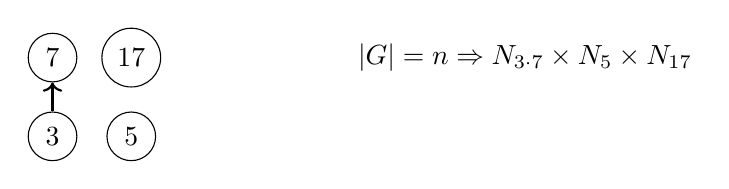
\begin{tikzpicture}
\node[circle,draw] (3) at (0,0) {$3$};
\node[circle,draw] (5) at (1,0) {$5$};
\node[circle,draw] (7) at (0,1) {$7$};
\node[circle,draw] (17) at (1,1) {$17$};

\draw[->,thick] (3) to (7);

\node at (6,1) {$|G|=n\Rightarrow N_{3\cdot 7}\times N_5\times N_{17}$};
\end{tikzpicture}
\end{center}
\end{block}


\end{frame}
    
\begin{frame}{Extending implications}

Factor $n$ into a \emph{direct hypergraph}.  (i) The Erd\H{o}s-P\'{a}lfy edges extended 
to factor as hyperedge, (ii) a list of exceptional divisors related finite nonabelian simple groups.

\begin{block}{Proposition}
    A group $G$ of order $n$ factors as 
\[N_0\ltimes (N_1\ltimes \cdots N_{\ell}),\] 
$|N_i|=n_i$, where $n_i$ is partitions of $\Gamma(n)$. 
\end{block}


\begin{block}{$n=5,810,340$}
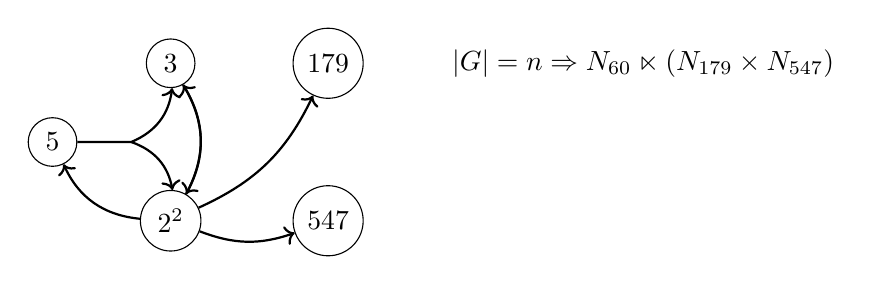
\begin{tikzpicture}
\node[circle,draw] (2) at (0,-1) {$2^2$};
\node[circle,draw] (3) at (0,1) {$3$};
\node[circle,draw] (5) at (-1.5,0) {$5$};
\node[circle,draw] (179) at (2,1) {$179$};
\node[circle,draw] (547) at (2,-1) {$547$};

\draw[->,thick] (2) to[bend right=30]  (3);
\draw[->,thick] (2) to[bend left=30]  (5);
\draw[->,thick] (2) to[bend right=20] (179);
\draw[->,thick] (2) to[bend right=20] (547);

\draw[->,thick] (5) to (-0.5,0) to[bend right=30] (3);
\draw[->,thick] (-0.5,0) to[bend left=30] (2);

\draw[->,thick] (3) to[bend left=30] (2);


\node at (6,1) {$|G|=n\Rightarrow N_{60}\ltimes (N_{179}\times N_{547})$};

\end{tikzpicture}
\end{block}


\end{frame}

\begin{frame}{}

\begin{center}
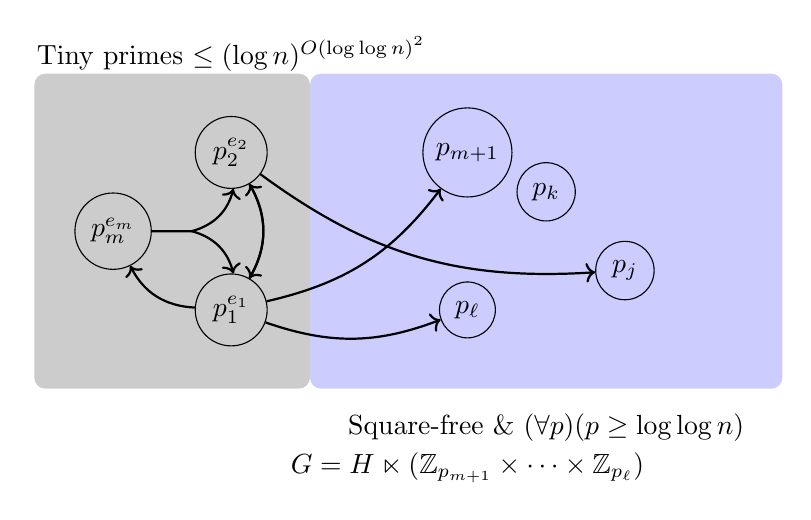
\begin{tikzpicture}

\fill[color=black!20,rounded corners] (-2.5,2) rectangle (1,-2);
\fill[color=blue!20,rounded corners] (1,2) rectangle (7,-2);

\node[circle,draw] (2) at (0,-1) {$p_1^{e_1}$};
\node[circle,draw] (3) at (0,1) {$p_2^{e_2}$};
\node[circle,draw] (5) at (-1.5,0) {$p_m^{e_{m}}$};
\node[circle,draw] (179) at (3,1) {$p_{m+1}$};
\node[circle,draw] (547) at (3,-1) {$p_{\ell}$};
\node[circle,draw] (1949) at (4,0.5) {$p_{k}$};
\node[circle,draw] (7893) at (5,-0.5) {$p_{j}$};



\draw[->,thick] (2) to[bend right=30]  (3);
\draw[->,thick] (2) to[bend left=30]  (5);
\draw[->,thick] (2) to[bend right=20] (179);
\draw[->,thick] (2) to[bend right=20] (547);

\draw[->,thick] (5) to (-0.5,0) to[bend right=30] (3);
\draw[->,thick] (-0.5,0) to[bend left=30] (2);

\draw[->,thick] (3) to[bend left=30] (2);

\draw[->,thick] (3) to[bend right=20] (7893);

\node at (0,2.25) {Tiny primes $\leq (\log n)^{O(\log \log n)^2}$};
\node at (4,-2.5) {Square-free \& $(\forall p)(p\geq \log \log n)$};
        
\node at (3,-3) {$G=H\ltimes (\mathbb{Z}_{p_{m+1}}\times\cdots \times \mathbb{Z}_{p_{\ell}})$};
\end{tikzpicture}    
\end{center}

\end{frame}
% \begin{frame}{}

% \begin{block}{Theorem.}
% A positive density of positive integers $n$ has $\Gamma(n)$ such 
% that the 
% \end{block}

% \end{frame}

% \begin{frame}{Most integers factor like this}

    
% \begin{tikzpicture}
% \node[circle,draw] (3) at (0,0) {$3$};
% \node[circle,draw] (31) at (1,1) {$31$};
% \node[circle,draw] (137) at (1,-1) {$137$};
% \node[circle,draw] (379) at (2,-1) {$379$};
% \node[circle,draw] (1949) at (3,0) {$1949$};

% \draw[->,thick] (3) to[bend left=30] (0,0.5) to[bend right=30] (31);
% \draw[->,thick] (3) to[bend left=30] (0,0.5) to[bend right=30] (31);
% % \draw[->,thick] (0,0.5) to[bend left=30] (5);
% % \draw[->,thick] (0,0.5) to[bend right=20] (541);

% % \draw[->,thick] (5) to[bend right=30] (-0.25,-0.5) to[bend right=30] (3);
% % \draw[->,thick] (-0.25,-0.5) to[bend left=30] (2);

% % \draw[->,thick] (3) to[bend right=30] (2);


% % \node at (6,1) {$|G|=n\Rightarrow N_{60}\ltimes N_{541}$};

% \end{tikzpicture}
    
% \end{frame}

\end{document}